% !TeX spellcheck = en_US
%\documentclass[11pt,a4paper]{article}
\documentclass[11pt
  , a4paper
  , article
  , oneside
%  , twoside
%  , draft
]{memoir}

\usepackage{control}
\usepackage{kotex}
\usepackage[numbers]{natbib}
%\usepackage[pdftex]{graphicx}
%\DeclareGraphicsExtensions{.pdf,.png,.jpg}
\begin{document}

\newcommand{\technumber}{
  Digital Signal Processing using MATLAB\\
  Document 1: 2016-03-26}
\title{\textbf{Digital Signal Processing: 실습 3 \\
		제2장 이산시간 신호 및 시스템 - 2 \\}}

\author{이상일\thanks{silee7103@ibs.re.kr} \\

  학번: 201460437\\
  Computer Engineering, Chungnam National University 
}
\date{\today}

\renewcommand{\maketitlehooka}{\begin{flushright}\textsf{\technumber}\end{flushright}}
%\renewcommand{\maketitlehookb}{\centering\textsf{\subtitle}}
%\renewcommand{\maketitlehookc}{C}
%\renewcommand{\maketitlehookd}{D}

\maketitle

\begin{abstract}
MATLAB을 사용한 Digital Signal Processing에 대한 실습과제에 대한 Documents를 구성한다.
\end{abstract}

\chapter{Example 2-9:}

\begin{lstlisting}[style=termstyle]
% Example 2.9

x = [3, 11, 7, 0, -1, 4, 2];
nx = [-3: 3];
h = [2, 3, 0, -5, 2, 1];
nh = [-1: 4];
[y,ny] = conv_m(x,nx,h,nh)
\end{lstlisting}

\begin{figure}[h!]
	\centering
	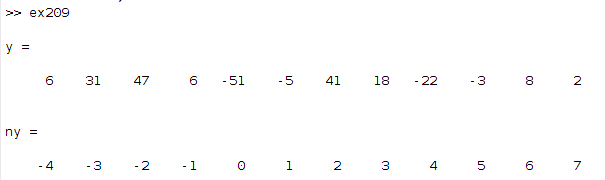
\includegraphics[width=0.7\textwidth,height=0.2\textwidth]{./images/ex209.png}
	\caption{Example 2.09 Result}
	\label{fig:Example 2.09 Result}
\end{figure}

\clearpage

\chapter{Example 2-10:}

\begin{lstlisting}[style=termstyle]
% Example 2.10
% noise sequence 1
x = [3, 11, 7, 0, -1, 4, 2]; nx=[-3:3]; % given signal x(n)
[y,ny] = sigshift(x,nx,2);              % obtain x(n-2)
w = randn(1,length(y)); nw = ny;        % generate w(n)
[y,ny] = sigadd(y,ny,w,nw);             % obtain y(n) = x(n-2) + w(n)
[x,nx] = sigfold(x,nx);                 % obtain x(-n)
[rxy,nrxy] = conv_m(y,ny,x,nx);         % cross-corrlation
subplot(1,1,1)
subplot(2,1,1);stem(nrxy,rxy)
axis([-4,8,-50,250]);xlabel('lag variable l')
ylabel('rxy');title('Crosscorrelation: noise sequence 1')

% noise sequence 2
x = [3, 11, 7, 0, -1, 4, 2]; nx=[-3:3]; % given signal x(n)
[y,ny] = sigshift(x,nx,2);              % obtain x(n-2)
w = randn(1,length(y)); nw = ny;        % generate w(n)
[y,ny] = sigadd(y,ny,w,nw);             % obtain y(n) = x(n-2) + w(n)
[x,nx] = sigfold(x,nx);                 % obtain x(-n)
[rxy,nrxy] = conv_m(y,ny,x,nx);         % cross-corrlation
subplot(2,1,2);stem(nrxy,rxy)
axis([-4,8,-50,250]);xlabel('lag variable l')
ylabel('rxy');title('Crosscorrelation: noise sequence 2')
\end{lstlisting}

\begin{figure}[h!]
	\centering
	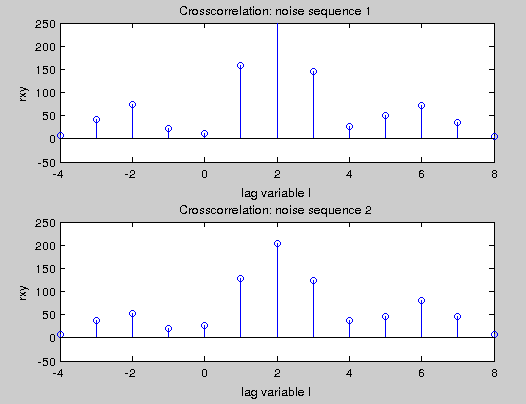
\includegraphics[width=0.7\textwidth,height=0.5\textwidth]{./images/ex210.png}
	\caption{Example 2.10 Result}
	\label{fig:Example 2.10 Result}
\end{figure}

\clearpage

\chapter{Example 2-11:}
\begin{lstlisting}[style=termstyle]
% Matlab Example 2.11;

a=[1,-1,0.9];b=1;

% Part a)
x=impseq(0,-20,120);n=[-20:120];
h=filter(b,a,x);
subplot(2,1,1);stem(n,h)
axis([-20,120,-1.1,1.1])
title('Impulse Response');xlabel('n');ylabel('h(n)')


% Part b)

x=stepseq(0,-20,120);
s=filter(b,a,x);
subplot(2,1,2);stem(n,s)
axis([-20,120,-.5,2.5])
title('Step Response');xlabel('n');ylabel('s(n)')

%print -deps2 ex021000.eps

% Part c)
sum(abs(h))
z=roots(a);
magz=abs(z)

\end{lstlisting}

\begin{figure}[h!]
	\centering
	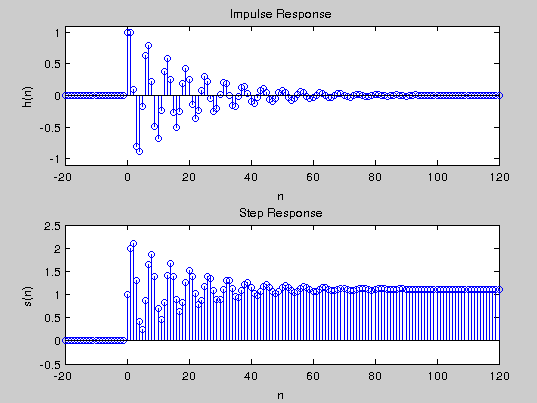
\includegraphics[width=0.7\textwidth,height=0.35\textwidth]{./images/ex211.png}
%	\caption{Example 2.11 Result}
	\label{fig:Example 2.11 Result}
\end{figure}

\begin{figure}[h!]
	\centering
	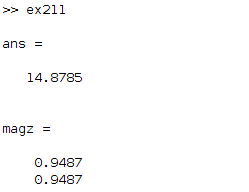
\includegraphics[width=0.45\textwidth,height=0.2\textwidth]{./images/ex211-1.png}
	\caption{Example 2.11 Result}
	\label{fig:Example 2.11-1 Result}
\end{figure}

\clearpage

\chapter{Example 2-12:}
\begin{lstlisting}[style=termstyle]
% Example 2.12

b = [1]; a = [1,-0.9];
n = -5:50; x = stepseq(0,-5,50) - stepseq(10,-5,50);
y = filter(b,a,x);
subplot(1,1,1);
subplot(2,1,2); stem(n,y); title('Output sequence')
xlabel('n'); ylabel('y(n)'); axis([-5,50,-0.5,8])

\end{lstlisting}

\begin{figure}[h!]
	\centering
	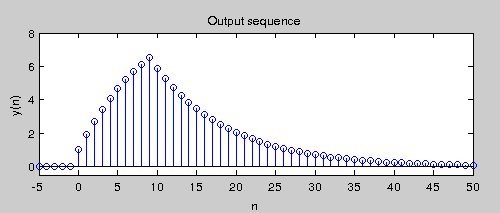
\includegraphics{./images/ex212.png}
	\caption{Example 2.12 Result}
	\label{fig:Example 2.12 Result}
\end{figure}

\chapter{Problem 2.4:}
\begin{lstlisting}[style=termstyle]
% Problem 2.4
% dnsample.m
function[y,m]=dnsample(x,n,M)
m=[integer(n(1),M):integer(n(length(n)),M)];
y=zeros(size(m));
for i=min(m):max(m)
y(i-min(m)+1)=x(M*i-min(n)+1);
end
\end{lstlisting}

\chapter{Problem 2.14:}
\begin{lstlisting}[style=termstyle]
% Problem 2.14
% conv_tp.m

function [y,H]=conv_tp(h,x)
% Linear Convolution using Toeplitz Matrix
% ----------------------------------------
% [y,H] = conv_tp(h,x)
% y = output sequence in column vector form
% H = Toeplitz matrix corresponding to sequence h so that y = Hx
% h = Impulse response sequence in column vector form
% x = input sequence in column vector form

Nx = length(x); Nh = length(h);
hc=[h; zeros(Nx-1, 1)];
hr=[h(1),zeros(1,Nx-1)];
H=toeplitz(hc,hr);
y=H*x;
end

\end{lstlisting}


\end{document}

